\section{Roisin}
\section{The Potential for Rooftop Photovoltaics}
\par
 If the federal government initiates large-scale deployment of rooftop PVs on federal buildings, the increase in demand would lower the cost of solar PVs. The extent to which federal demand for rooftop solar can effect the PV market hinges on the amount of federal electricity demand which can be met by rooftop photovoltaics. Furthermore, the viability of federal PV rooftop installations the cost and profitability of PV technologies must be considered. This study characterizes the potential energy generation, cost and profitabiliy of rooftop PV for federal buildings.

The energy generated with rooftop PV can vary based on physical parameters including rooftop size, and solar irradiance.  In order to approximate the total solar potential across all federal buildings a detailed dataset of existing federal buildings is required. The GSA provides a digital inventory of all leased and federally owned buildings managed in the United States \cite{roisin}{rtl9}. The federal building inventory includes street addresses, zip codes and gross building area. The approximately 1500 federally owned buildings within the GSA inventory are evaluated for rooftop potential and collectively represent the rooftop potential for federal properties.

\par
To calculate the energy potential of an installed system, the solar insolation on the rooftop surface is computed as function of the solar irradiance, surface area, and exposure time. The amount of solar energy that is converted by the solar panel can then be computed by including the efficiency of the technology and performance ratio of the system. The available solar resource is a key factor for PV energy output and subsequent system profitability. In the US, solar energy varies from North to South, East to West and on smaller scales due to altitude and regional climate. Figure \ref{fig:rtl_pic3}, taken from NREL, shows the variability in solar resources across the country and within state boundaries.  To obtain an accurate approximation of PV rooftop potential, it was critical to utilize the high-resolution values for solar irradiance at each federal building. 

\begin{wrapfigure}{r}{0.7\textwidth}
  \begin{center}
    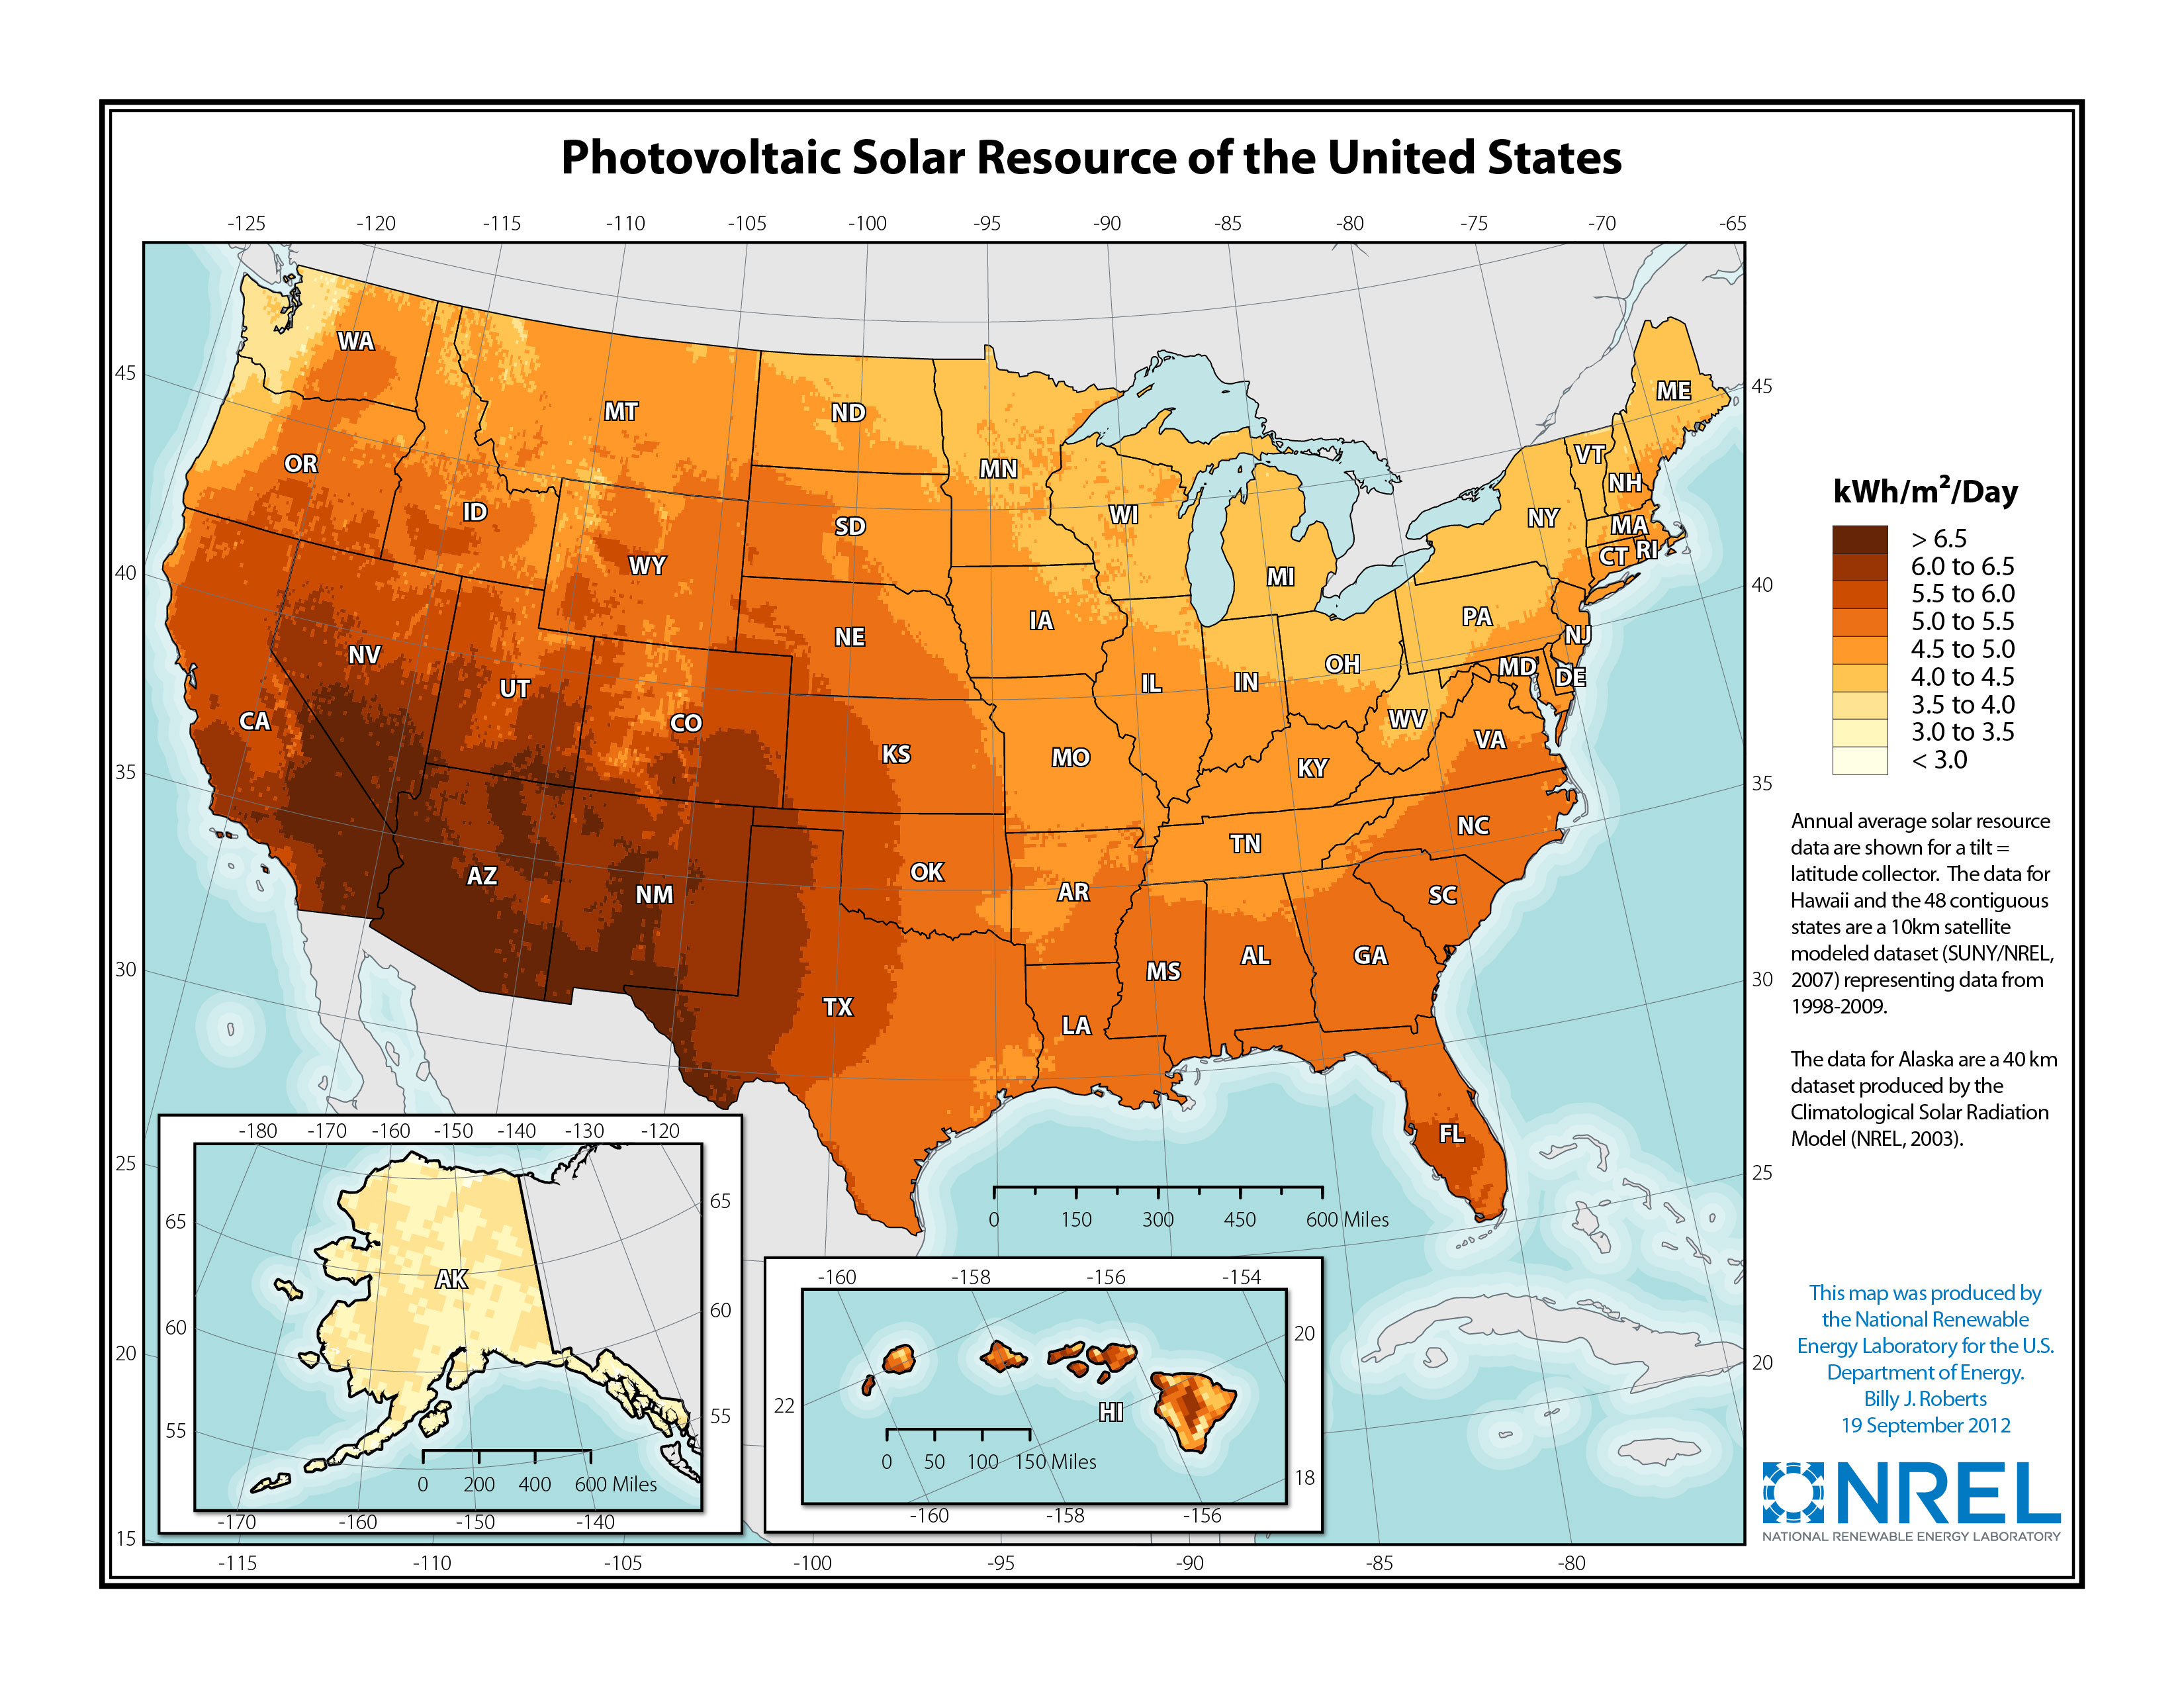
\includegraphics[width=0.68\textwidth]{pics/rtl_pic3}
  \end{center}
  \caption{source: NREL}
\label{fig:rtl_pic3}
\end{wrapfigure}

The Global Horizontal Irradiance (GHI) for each state and zip code in the US was obtained from NRELs 10-kilometer Solar Data \cite{roisin}{rtl10}. The annual average GHI or total solar radiation, is used determine the solar potential for Flat-pane rooftop PVs at that location. GHI is the sum of the Direct Normal Irradiance (DNI) and Diffuse Horizontal Irradiance (DHI) and ground-reflected radiation.  A procedure known as record linkage, data matching or data merging is used to pair solar insolation values with federal buildings based on their 5-digit zip codes.  In other words, the 5-digit zip code is used to uniquely identify common entries in the GSA building dataset and the 10-kilometer Solar Dataset. For approximately 170 missing GHI values, the state-level GHI value was instead referenced. After matches are made linking GHI values with federal buildings, a new dataset is generated containing both the federal building data and corresponding GHI values. Record matching is implemented in Microsoft Excel using the match and index functions.  The entry matching procedure is also used to obtain state-level electricity rates for each building which is discussed in further sections.  
\par
For a single rooftop PV installation, the energy generated over $N_{days}$ is calculated by:  

\begin{equation}
E_{gen}=A_{eff}*GHI*N_{days}*\eta*P 
\end{equation}

where $E_{gen}$ is the annual electricity production in $kWh$, $A_{eff}$ is the surface area of the solar cells in $m^2$, $GHI$ is the total solar radiation in $kWh/m^{2}/day$, $\eta$ is the PV efficiency, and $P$ is the performance ratio of the solar panels \cite{rtl8}. The effective surface area represents the collective roof area covered by PV panels on a rooftop and is assumed to be 75\% of the roof area. The amount of energy that can be turned into electricity by PVs is effected by the efficiency of the panel, $\eta$, as well as the performance ratio, $P$, a quantity which accounts for losses from dust, inclination, and surface irregularities. 
\par
For each of the 1500 federal buildings, the yearly generation potential of PV modules covering the available rooftop area is computed.  Local GHI values are used in the calculation and rooftop area is approximated from GSA measurements of each of the buildings. The histogram of building gross areas shown in figure \ref{fig:rtl_pic1} reveals most federal buildings to be small, 1 or 2 story structures. 
\begin{wrapfigure}{l}{0.7\textwidth}
  \begin{center}
    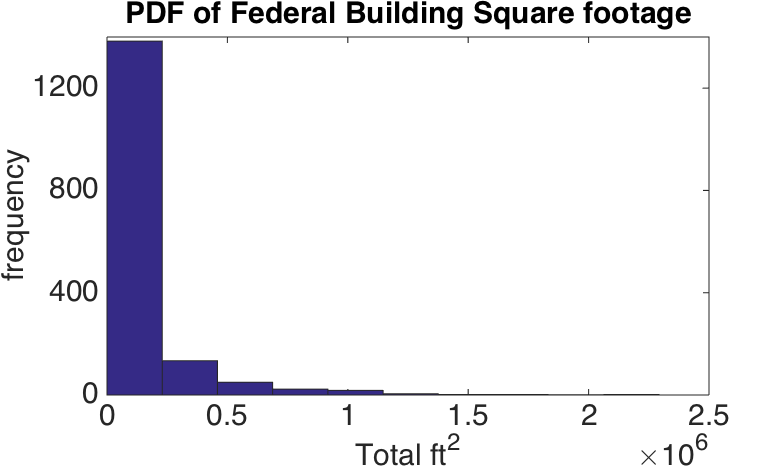
\includegraphics[width=0.68\textwidth]{pics/rtl_pic1}
  \end{center}
\label{fig:rtl_pic1}
\end{wrapfigure}

For the majority of buildings, the roof area assumed to be equal to building gross area. For buildings greater that 25,000 $ft^2$, it is likely that the building has multiple stories thus a maximium roof area of 25,000 $ft^2$ is used. The upper threshold prevents any severe overestimation of rooftop availability. A performance ratio of 75\% and a PV efficiency of 16\% are assumed to represent the installed solar technology \cite{roisin}{rtl8}. While the yearly generation was computed for each building, the average and total values are supplied in this report. Collectively the 1500 federal buildings are approximated to have 1,636,152 $m^2$ of effective rooftop area which can be harnessed to supply 317,058,200 $kWh/year$ of electricity. The average federal building is found to have an effective rooftop area of 1,073 $m^2$ with which PVs can generate 207,907 $kWh/year$.
\par 

The potential benefit and cost of installing PV on rooftops presents a trade-off between the up-front installation costs and the long-term savings in building energy costs from renewable energy generation. To compute the cost of the system we must consider differences in market PV costs, operation and maintence costs over the systems lifetime and in the different building locations. Due to the lack of data availability on installed PV prices, the most recent cost of commercial rooftop PV is used to evaluate the upfront cost of installation---3,819 dollars per $kW$ \cite{roisin}{rtl4}. Using the cost of installation and the approximated rooftop system capacities ($kW$), the system cost is obtained for each building. 
\par
The electricity rates used to compute the energy savings per building represent the `Average Retail Price of Electricity to Ultimate Customers by End-Use Sector by State' \cite{roisin}{rtl3} and are linked to each building using the 2-letter state acronym and matching procedure outlined above. The yearly savings in building energy costs is computed by multiplying the $kWh$ of PV generation with the market rates of electricity in dollars per $kWh$. To account for the cost of operation and maintence of the system a penalty of .2\% of the upfront capital investment is subtracted from the yearly savings estimate. Finally, the payback period is determined by the ratio of upfront system cost (dollars) over the annual savings (dollars). 
\par
The histogram of the all PV payback periods are shown in Figure \ref{fig:rtl_pic4}. The payback periods for the 1500 buidlings range between 5 and 40 years, with an average of 24 years.
\begin{figure}
  \centering
    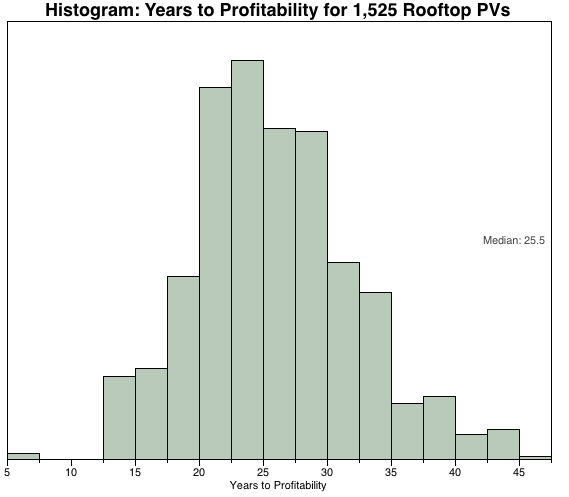
\includegraphics[width=0.7\textwidth]{pics/rtl_pic4}
  \label{fig:rtl_pic4}
\end{figure}
 Summary variables of the cost analysis for 2 deployment scenarios are provided in Figure \ref{fig:rtl_pic2}. In each case, the price of electricity is assumed to remain fixed over time. For scenario 1, the cost and profitability calculations are estimated for all 1500 buildings, the average values for a single building and for all buildings are listed in columns 1 and 2 respectively. For the average federal building, rooftop PV installations will breakeven after 24 years and generate 20,220 dollars in energy savings thereafter.  The economic variables are also evaluated for a second scenario in which half of the federally owned buildings are fitted with rooftop solar---those with the shortest profitability timelines. The average and total values for the most profitable half of federal builidings are shown in columns 4 and 5. For the most productive half of federal rooftops, PV installations breakeven on average after 22 years and save 25,137 dollars annualy per building. If PV were installed on half of federal buildings, after 25 years all installations would break even and save 14,957,037 dollars a year for the remaining system lifetime. 

\begin{figure}
  \centering
    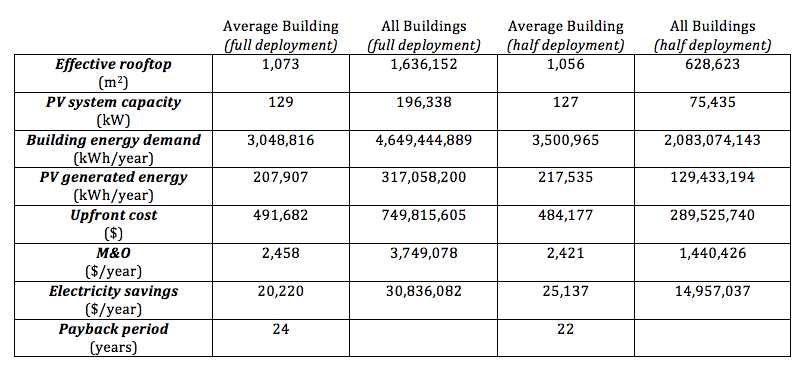
\includegraphics[width=0.98\textwidth]{pics/rtl_pic2}
  \caption{Summary of key variables for the full deployment of PV on (1) all federal rooftops and (2) the most profitable half denoted full and half deployment respectively.}
  \label{fig:rtl_pic2}
\end{figure}

By computing the rooftop potential and performing a cost analysis of rooftop PVs for each federal building, we establish a database of economic metrics which can be used to inform the policy deployment and building prioritization. The economic analysis demonstrates that rooftop solar is not only feasible but profitable for the majority of existing federal buildings.
